\documentclass[11pt]{article}

\usepackage{graphicx}
\usepackage{courier}
\usepackage{underscore}

\title{Turing Machine Format Explanation}
\author{Adam Yedidia}

\begin{document}
    
\maketitle

This document explains how to understand generated Turing machines, which can be found at: \\ \\
\texttt{parsimony/src/tm/tm2/tm2_files} \\
or \\
\texttt{parsimony/src/tm/tm4/tm4_files} \\ \\
depending on whether the machine's alphabet size is 2 or 4. \\

The following is an example of the file format of the single-tape, 4-symbol Turing machine output by the compiler. \\

Let us suppose that the Turing machine has three states. The four symbols in the Turing machine's alphabet are ``\texttt{\_},'' ``\texttt{1},'' ``\texttt{E},'' and ``texttt{H}'' The first state's name is ``\texttt{StateOne},'' the second state's name is ``\texttt{StateTwo},'' and the third state's name is ``\texttt{StateThree}.'' The first tape's name is ``\texttt{TapeA},'' and the second tape's name is ``\texttt{TapeB}.'' \\

\texttt{StateOne} is associated with \texttt{TapeA}. \texttt{StateTwo} is associated with \texttt{TapeB}. \texttt{StateThree} is associated with \texttt{TapeA}. \\

Each line defining the Turing machine's behavior in a given state is written as follows: \\

\texttt{[symbol read] -> [next state]; [direction]; [symbol written]} \\

In the actual Turing machine text file, [next state] is replaced by the state that the Turing machine would enter if it read the symbol [symbol read], [direction] is one of \{\texttt{R, L, -}\} and indicates the direction the head would move in, and [symbol written] is one of \{\texttt{\_, 1, E}\} and indicates the symbol that is written on the tape. Note that in the higher-level, multi-tape 3-symbol Turing machine, as indicated by the \texttt{-} symbol, the head can remain in place, (unlike the lowest-level Turing machine around which the Busy Beaver function is defined, where it cannot). \\

Figure~\ref{fig:tmexample} shows an example of such a Turing machine file.

\begin{figure} 
\begin{center} 
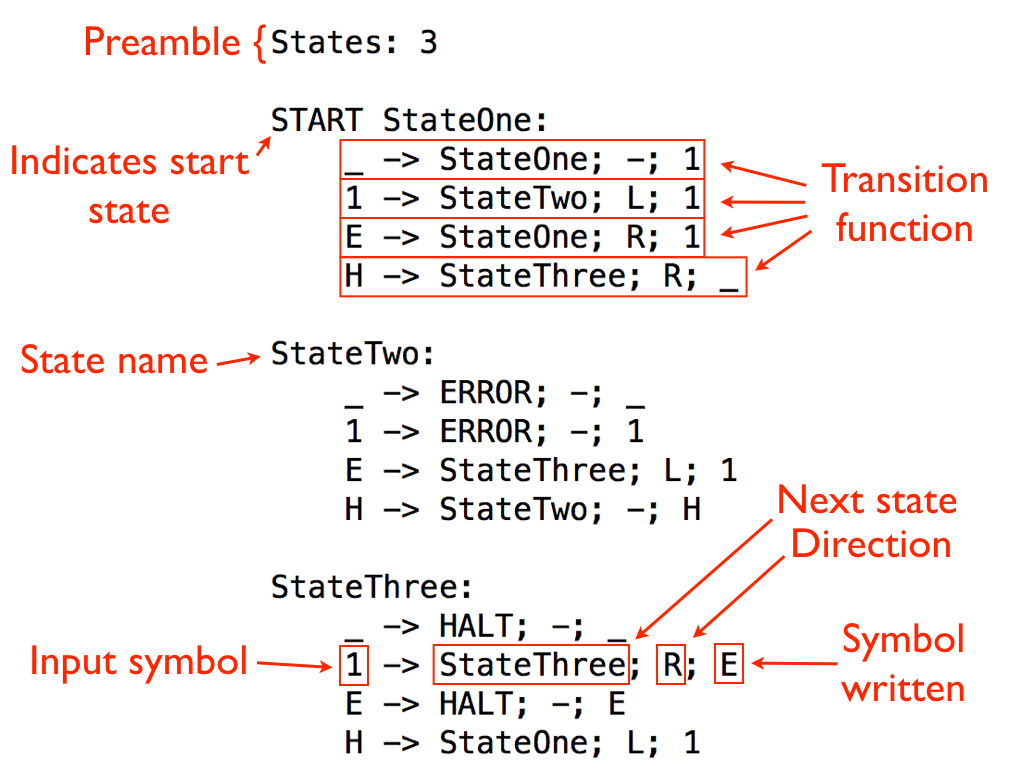
\includegraphics[scale=0.4]{figs/annotatedtm.png} 
\caption{This is an example of a multi-tape Turing machine file. The notes in red are explanations of the meanings of the various parts of the Turing machine file. \label{fig:tmexample}} 
\end{center} 
\end{figure}

\end{document}